\section{Do Desenho à Simulação}

Nos Relatórios I e II foram apresentadas imagens do design do BROV. Até então, os outros componentes do cenário de simulação ainda não haviam sido modelados. Dessa forma, a primeira atividade do Relatório III foi a finalização da modelagem 3D dos itens: objeto, boia e SBL. 

Para a missão de resgate, o objeto escolhido foi uma moeda de um real, fixado em um lastro, conforme mostra a Figura \ref{fig:object3}. O lastro é composto por uma base maciça de aço, perfis quadrados e chapas para fixação de quatro ArUcos. Os ArUcos são utilizados para a confirmação da detecção da moeda quando o BROV se aproxima da localização desejada (\textit{fine-tuning}). A moeda, por sua vez, é fixada em uma haste metálica através de cola ou barbante. Quando o BROV confirma a detecção do ArUco onde está a moeda, ele se desloca até a moeda e a coleta através de uma haste metálica com um ímã na ponta (item não modelado). A hipótese é que a força de atração do ímã é superior à de fixação exercida pela cola ou barbante.

\begin{figure}[h]
	\centering
	\caption[Objeto a ser resgatado]{Objeto a ser resgatado}
	\label{fig:object3}
	\includegraphics[width=1\linewidth]{images/object3}\\
	\footnotesize Fonte: Autores
\end{figure}

O design da boia levou em consideração os aspectos de comunicação. Como pode ser visto na Figura \ref{fig:boia}, a parte na cor amarela indica uma antena para transmissão de dados via Wi-Fi e recepção via Bluetooth, enquanto que a parte submersa, representada pela cor cinza, corresponde ao transdutor ultrassônico utilizado para transmissão e recepção de dados. A parte vermelha acomoda toda a eletrônica e sistema de alimentação dos dois sistemas, e possui a maior parte do volume não preenchido.

\begin{figure}[h]
	\centering
	\caption[Boia utilizada para transmissão e recepção de dados]{Boia utilizada para transmissão e recepção de dados}
	\label{fig:boia}
	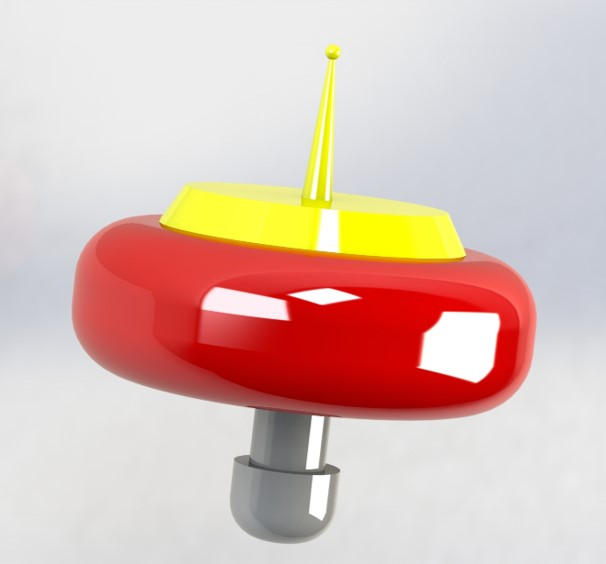
\includegraphics[width=0.6\linewidth]{images/boia}\\
	\footnotesize Fonte: Autores
\end{figure}

O sistema escolhido para a localização foi o SBL (do inglês \textit{short baseline}) e está representado pela Figura \ref{fig:sbl}. Ao todo, serão utilizados quatro transdutores em posições conhecidas, alimentados por uma bateria.

\begin{figure}[h]
	\centering
	\caption[Sistema SBL utilizado para localização]{Sistema SBL utilizado para localização}
	\label{fig:sbl}
	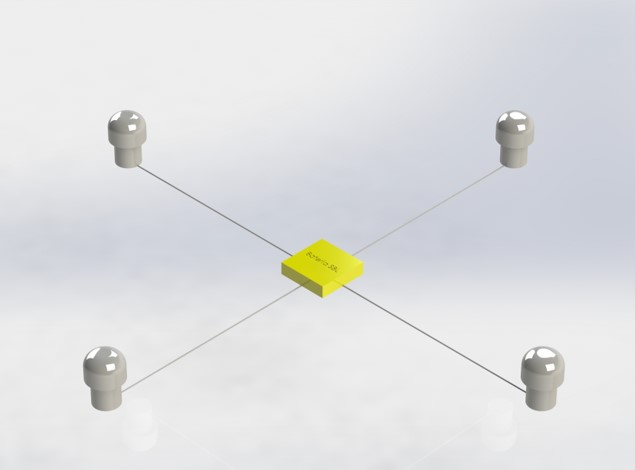
\includegraphics[width=0.7\linewidth]{images/sbl}\\
	\footnotesize Fonte: Autores
\end{figure}

A etapa subsequente foi exportar os dados de CAD, no formato .sldprt e .sldasm, para .stl e .dae, que são formatos aceitos pelo Ignition (software utilizado para simulação). Esses tipos arquivos aceitos pelo Ignition representam descrição de malha, que é a representação da superfície de um objeto 3D apenas com poligonos simples. A diferença entre os formatos .stl e .dae aceitos é que o primeiro não armazena informação de cor dos polígonos, diferentemente do segundo, que também consta com propriedades de reflexão, normais e textura da malha, que o torna mais pesado e custoso de ser processado do que o .stl. O Ignition trabalha com malhas para duas funcionalidades, aplicação da física e visualização. Dessa forma, se optou pela utilização do arquivo mais leve .stl para a simulação da física e a utilização do .dae com cores e texturas para a visualização. Ademais, se redesenenhou o veículo para a geração da malha .stl, visto que a compexidade de sua superfície demandava processamento que tornava a aplicação lenta nos computadores disponíveis para o projeto.

 A Figura \ref{fig:software-flow} resume o fluxo de softwares utilizados para o processo de conversão de CAD em malha. Como o Solidworks -- utilizado para modelagem 3D -- não fornece opção para exportar arquivos de .sldprt e .sldasm diretamente para .dae, optou-se por utilizar o Onshape e o Blender como softwares intermediários para geração desse tipo de arquivo e eventuais correções de escala e posicionamento do centro global de coordenadas.

\begin{figure}[h]
	\centering
	\caption[Fluxo de softwares utilizados]{Fluxo de softwares utilizados}
	\label{fig:software-flow}
	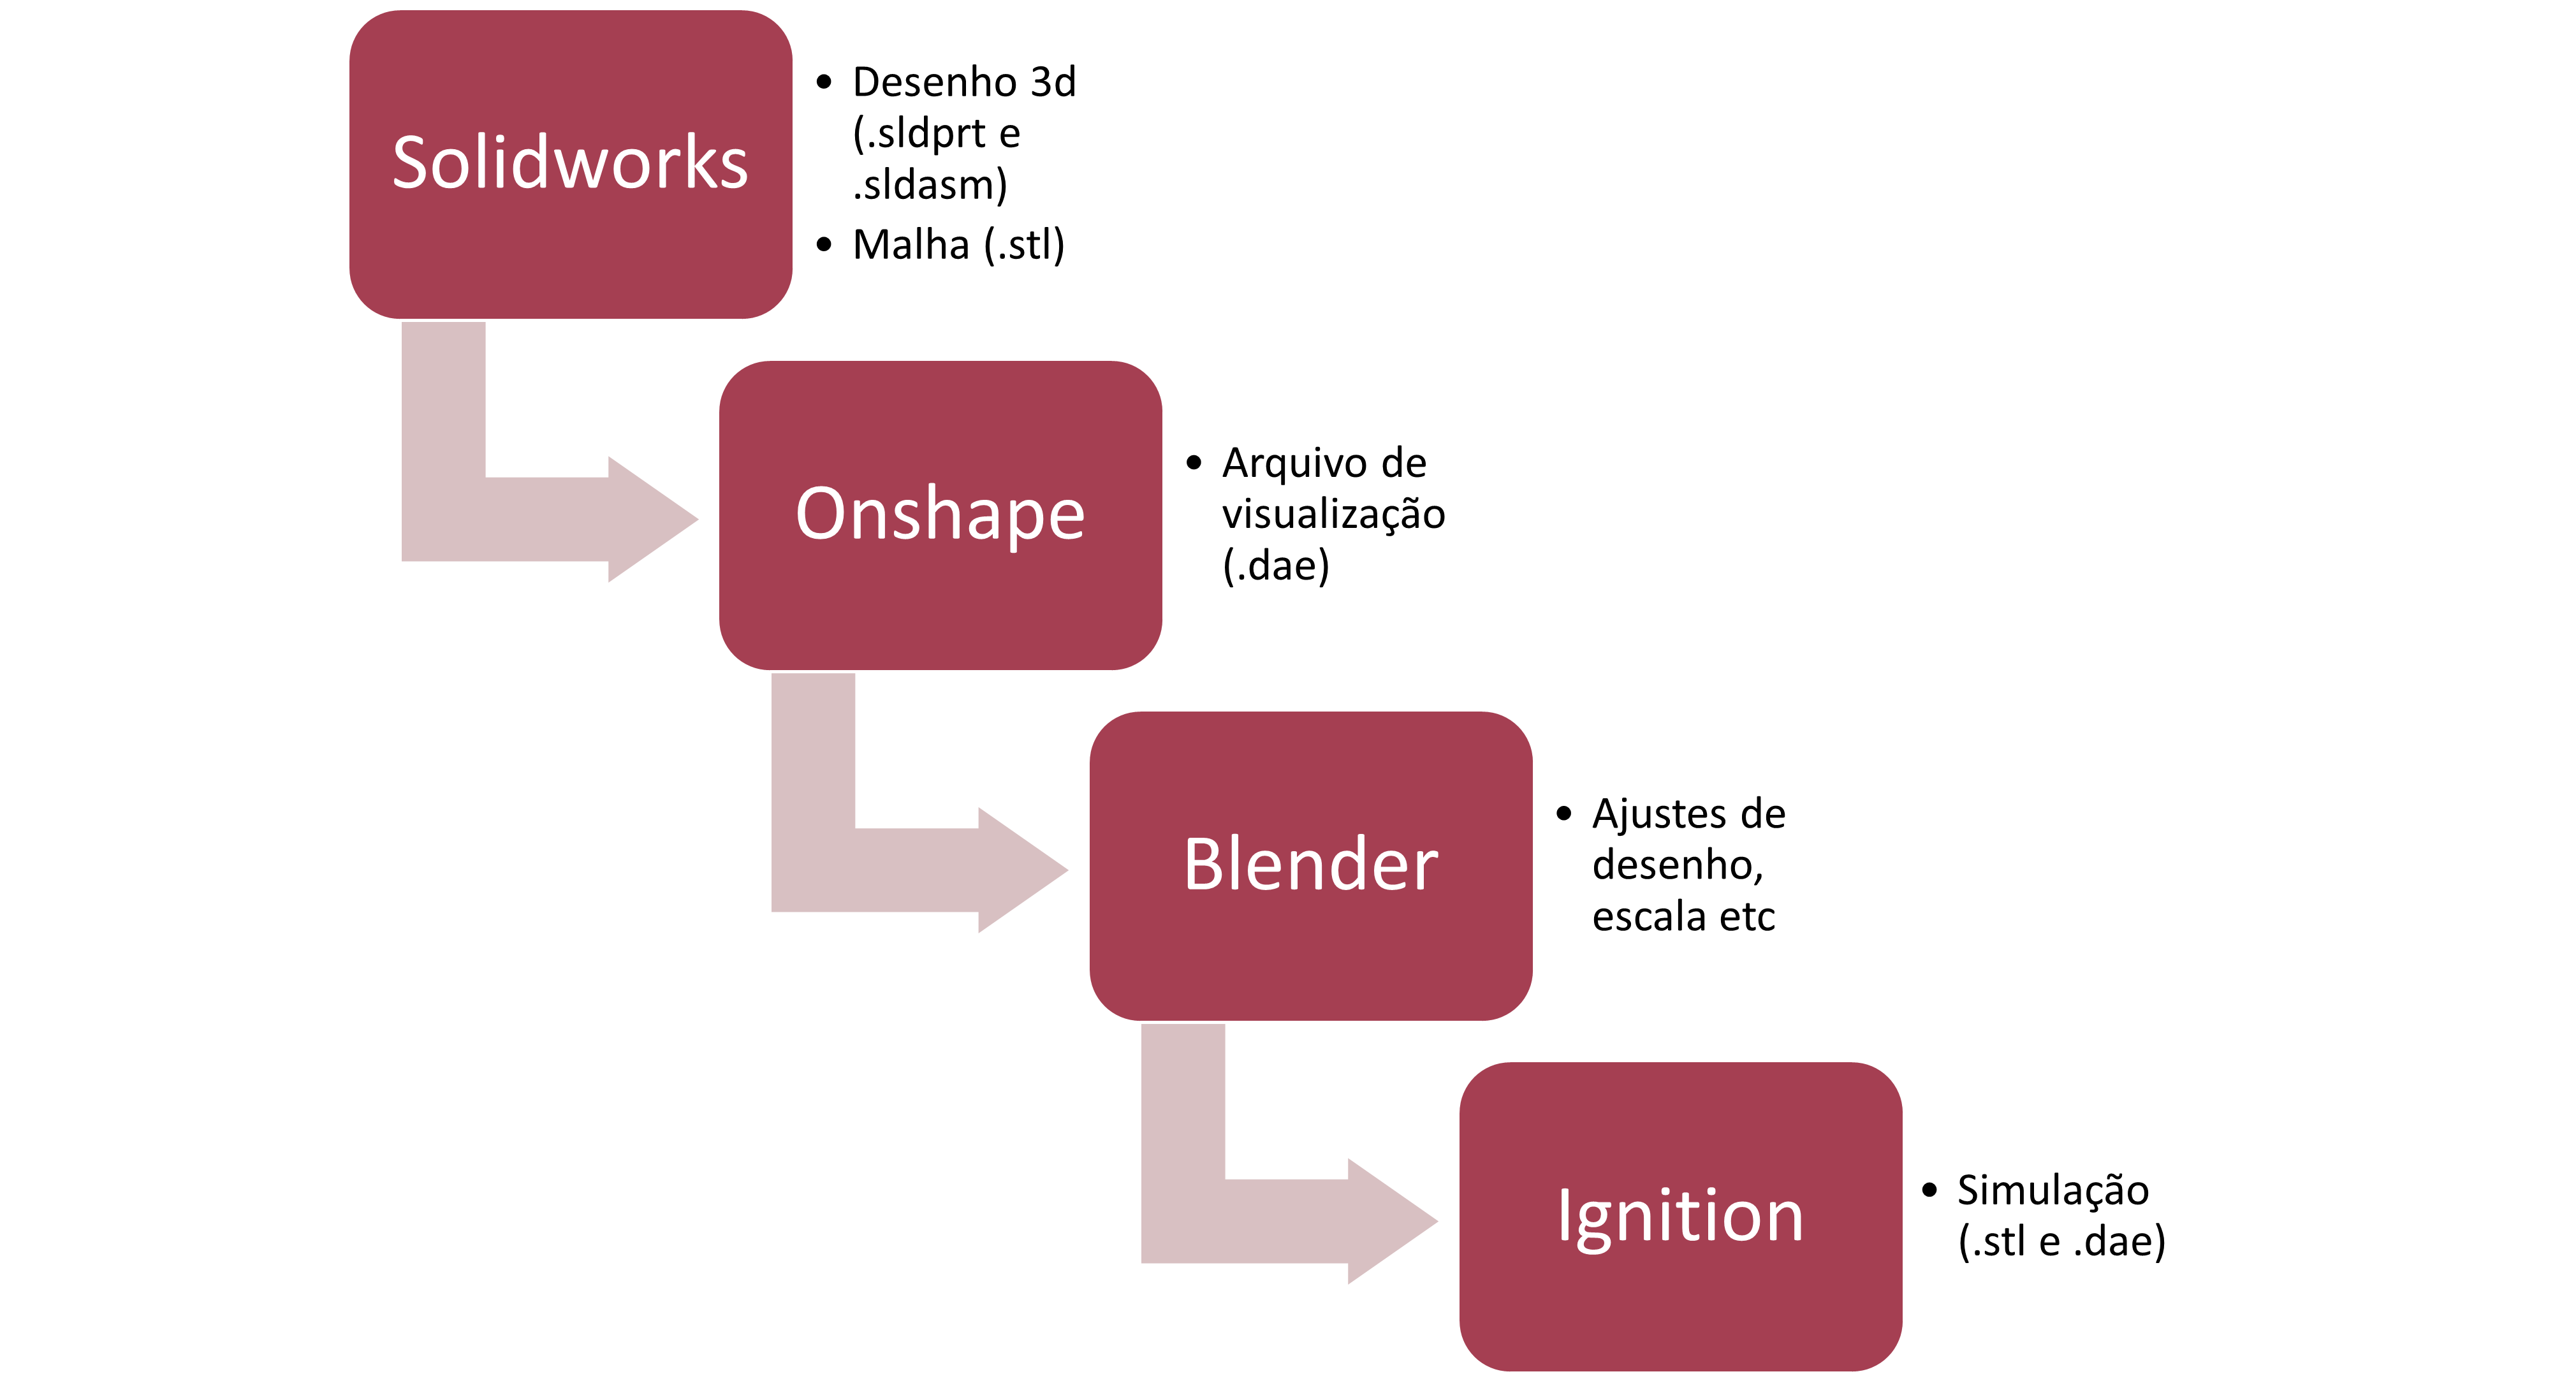
\includegraphics[width=1\linewidth]{images/software-flow}\\
	\footnotesize Fonte: Autores
\end{figure}


